The desktop application (see Figures~\ref{fig:desktop-app-running-signal-generation} and~\ref{fig:desktop-app-standby-eeg-measured}) was developed using the Electron framework, which allows for cross-platform compatibility and seamless integration with the underlying hardware. The application provides a user-friendly interface for configuring stimulation parameters, monitoring real-time data, and visualizing results.

\begin{figure}[H]
    \centering
    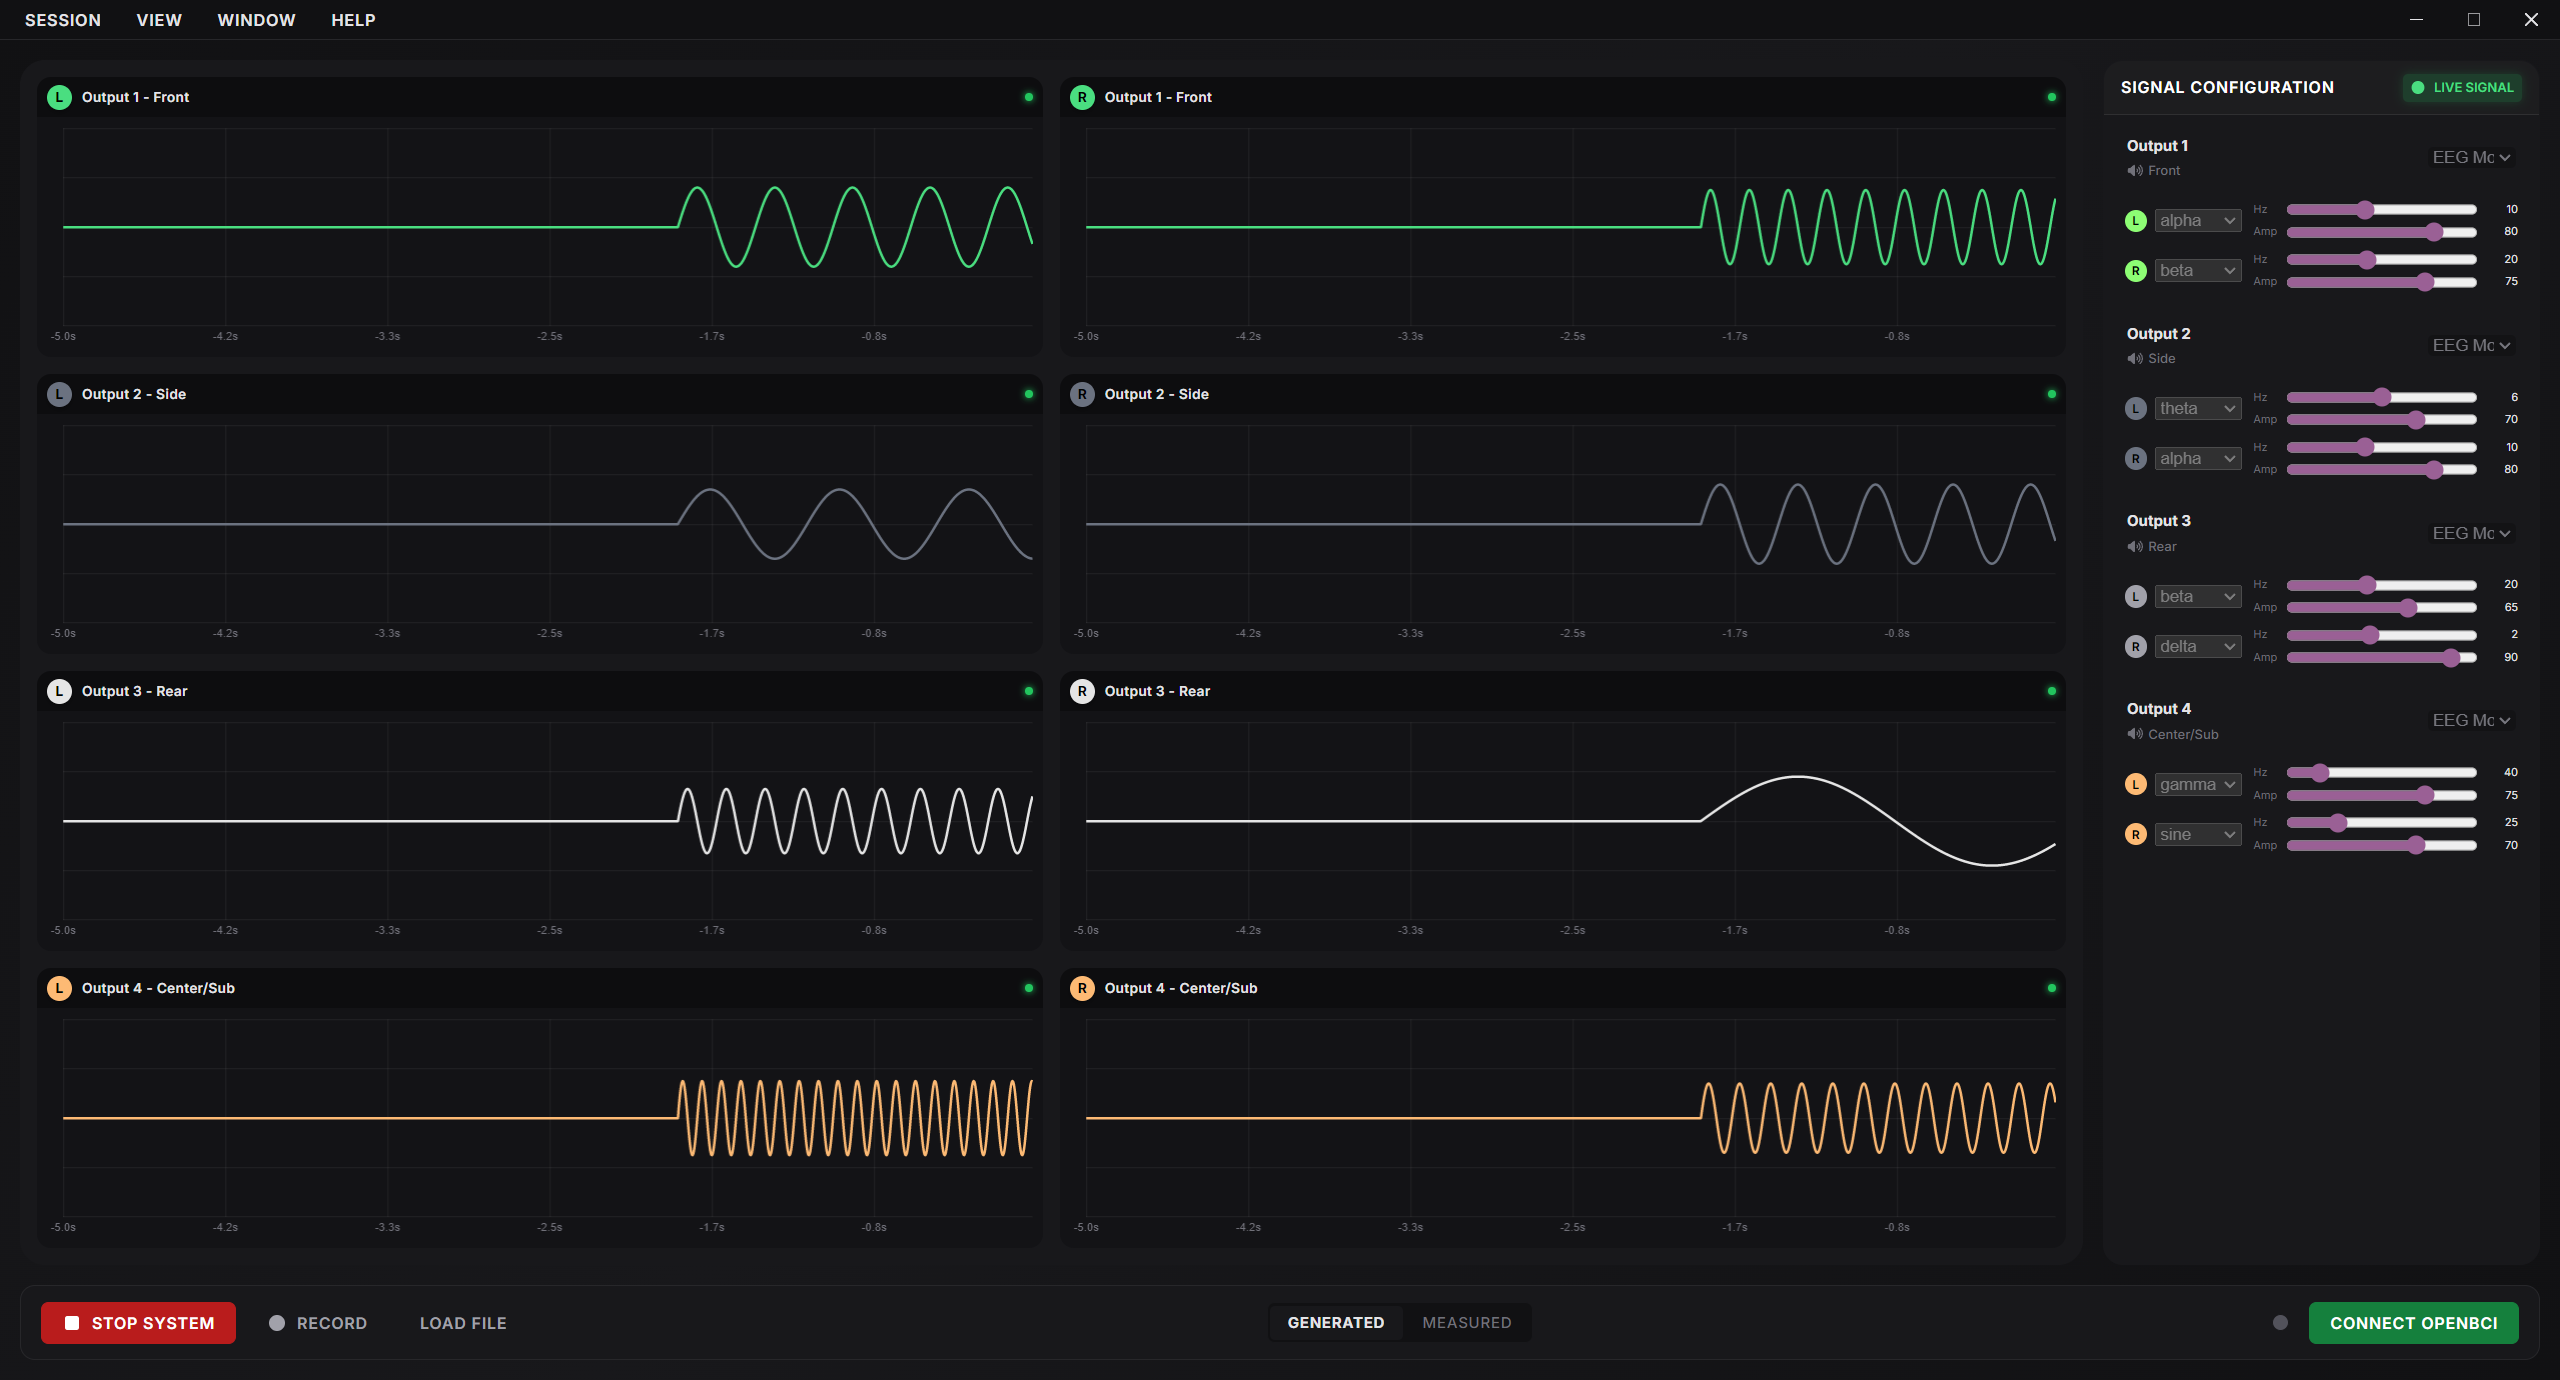
\includegraphics[width=0.6\textwidth]{../../02_Images/desktop-app-running-signal-generation.png}
    \caption[Desktop application running signal generation]{Desktop application running signal generation screen.}
    \label{fig:desktop-app-running-signal-generation}
\end{figure}

\begin{figure}[H]
    \centering
    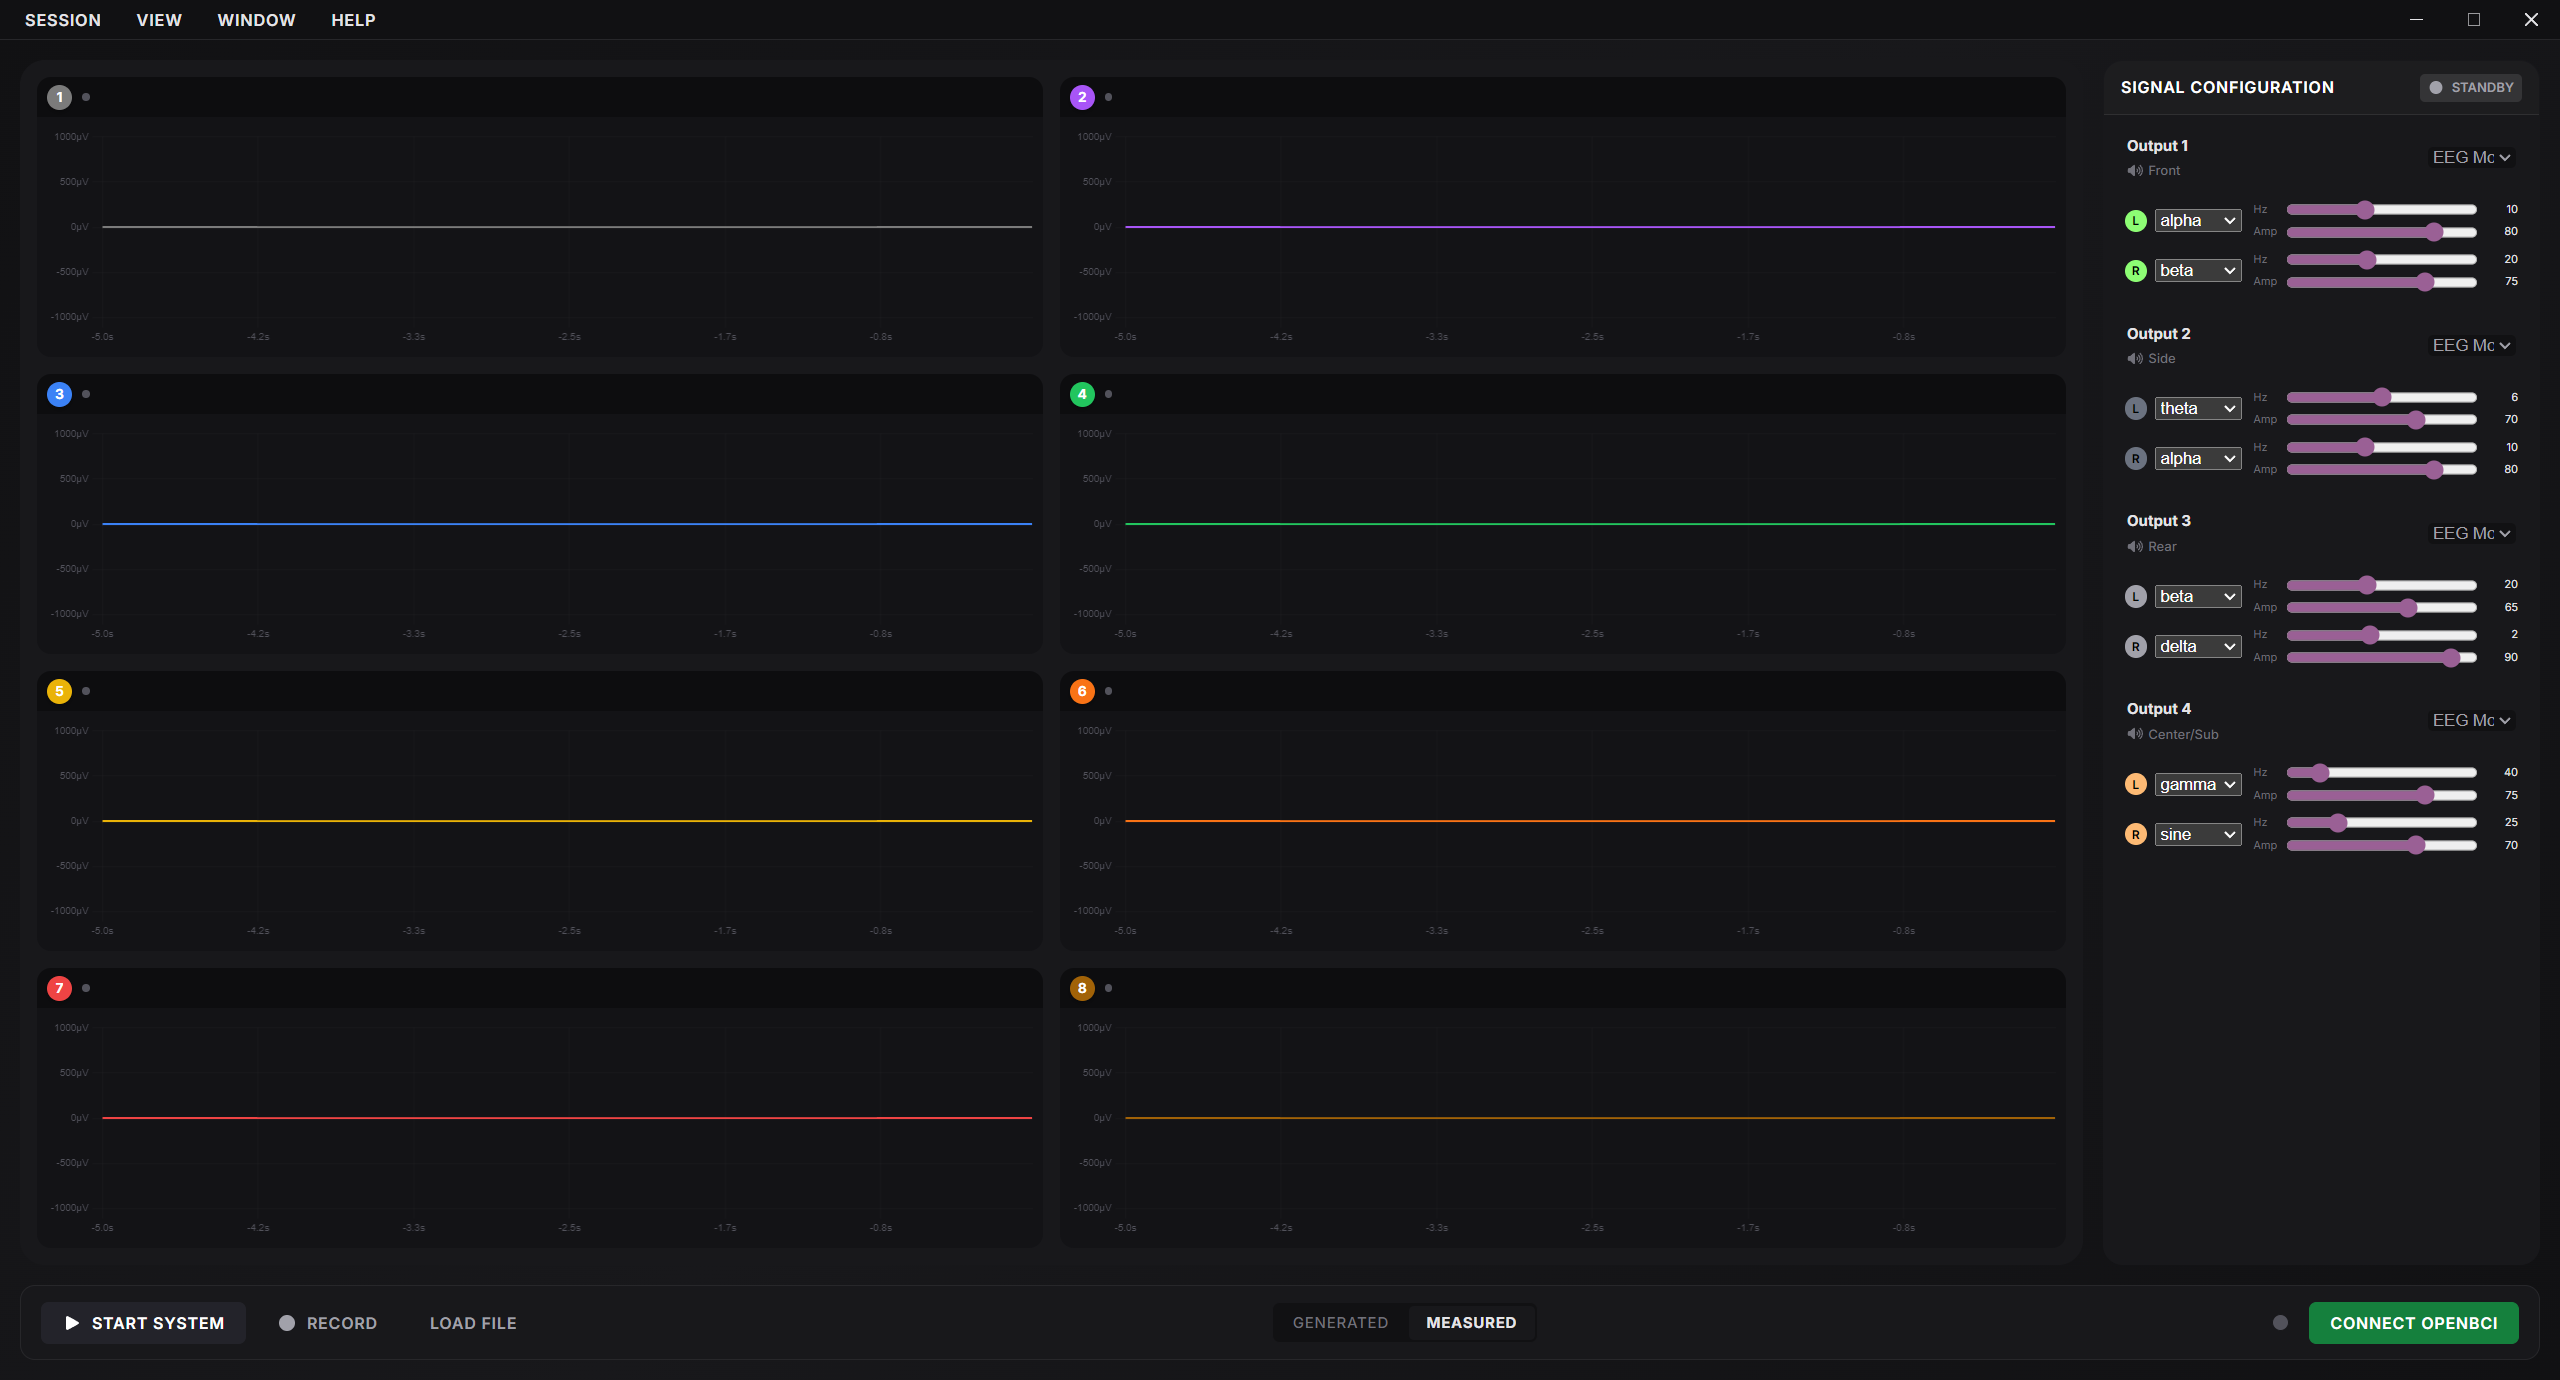
\includegraphics[width=0.6\textwidth]{../../02_Images/desktop-app-standby-eeg-measured.png}
    \caption[Desktop application standby EEG measured screen]{Desktop application standby EEG measured screen.}
    \label{fig:desktop-app-standby-eeg-measured}
\end{figure}

\nota{Falta screenshot de la app corriendo la medición EEG en tiempo real}